\documentclass{article}
\usepackage{amsfonts}
\usepackage{multicol}
\usepackage[utf8x]{inputenc}
\usepackage{graphicx}
\usepackage{geometry}
\geometry{a4paper, total={170mm, 237mm}, left=20mm, top=20mm}
 
\title{ {\Large \textbf{DÉMONSTRATION AUTOMATIQUE EN COQ}} }
\date{}
\author{Quentin Garchery}

\setlength{\parindent}{0cm}


\begin{document}

\maketitle
\thispagestyle{empty}

\begin{center}
\normalsize sous la direction de \\

\vspace{7mm}

\begin{multicols}{2}
\large{Chantal Keller} \\
Maître de Conférences\\
Université Paris-Sud \\

\large{Valentin Blot} \\
Post-doctorant\\
Université Paris-Sud
\end{multicols}

\vspace{15mm}

\Large{Stage au Laboratoire de Recherche en Informatique\\
Université Paris-Sud / CNRS}


\vfill

\normalsize 20 août 2018

\end{center}
\newpage



\section{Introduction}

\subsection{Méthodes formelles}

Les méthodes formelles rassemblent différents outils informatiques qui permettent de formuler des propriétés mathématiques puis de les vérifier. La validité du résultat vérifié ne dépend alors que de ce logiciel de vérification. C'est dans ce cadre que G. Gonthier et B. Werner ont prouvé, en Coq, le théorème des quatre couleurs.\\

Les méthodes formelles s'étendent à la preuve de programme: il s'agit alors de vérifier qu'un programme correspond à sa spécification et permet donc d'aug-menter sa robustesse et sa fiabilité.
L'importance de la correction des logiciels est mise en avant dans le cas des systèmes critiques : le premier lancement d'Ariane 5 (1996) s'est soldé par un échec dû à un bug logiciel. Le compilateur Compcert est un exemple de programme certifié, sa vérification a été effectuée en Coq.\\

Parmi ces outils de vérification, on s'intéressera aux assistants de preuves et aux prouveurs automatiques. 

\subsection{Assistants de preuve}

Les assistants de preuves tels que Coq sont des outils puissants qui permettent d'exprimer des théorèmes complexes puis de les vérifier de manière interactive. Ils proposent à un utilisateur de formuler son problème puis de le démontrer, le rôle principal de l'assistant de preuve étant alors de vérifier que la preuve fournie est correcte.  La confiance accordée à ces outils dépend de la compréhension que l'on peut avoir dans son noyau, étant donné que c'est la partie sur laquelle repose la vérification. Cette compréhension est facilitée lorsque l'implantation de la logique de ce noyau est de taille réduite. \\

Pour une propriété donnée, l'utilisateur doit donc fournir une preuve parfaitement rigoureuse et exhaustive de la propriété ce qui peut rendre le processus de vérification long et fastidieux.



\subsection{Prouveurs automatiques}

Les prouveurs automatiques, quant à eux, ne demandent pas de preuves de la part de l'utilisateur. L'effort de certification est alors réduit à la formalisation du problème et dans certains cas le prouveur donne une trace de son exécution appelée certificat. \\

En contrepartie, la logique d'un prouveur automatique est plus limitée et/ou la réponse en temps fini n'est pas garantie.

\subsection{Motivations}

Nous aimerions bénéficier de l'automatisation des prouveurs automatiques dans un système expressif et sûr comme les assistants de preuves. Cette étape est faite par SMTCoq initialement. \\

Nous aimerions aussi que le développement à l'aide de cette automatisation soit adapté aux assistants de preuves: les preuves sont modulaires et peuvent reposer sur des lemmes précédemment démontrés. Pendant mon stage, je me suis attaché à améliorer ce point.


\subsection{Contexte}

L'assistant de preuve que nous utiliserons est Coq, sa logique du noyau se fonde sur le Calcul Inductif des Constructions. \\

SMTCoq est un plugin pour Coq qui utilise différents prouveurs automatiques. C'est un outil modulaire dans le sens où il est possible de rajouter d'autres prouveurs automatiques, ceux-ci n'ayant pas nécessairement le même format d'entrée ni le même format de sortie. SMTCoq permet d'une part d'améliorer l'automatisation de Coq. En effet, les preuves générées automatiquement par les prouveurs sont ensuite utilisée pour des preuves dans Coq. D'autre part, cela permet de vérifier les certificats fournis par les prouveurs automatiques et donc d'augmenter la confiance que l'on a dans ces outils.


\section{Utilisation de Coq}

\subsection{Calcul Inductif des Constructions}

CIC \\
types dépendants

\subsection{Preuve par réflection calculatoire}

La preuve par réflection utilise l'égalité interne à Coq: deux termes sont considérés à réduction près. 
Aussi, à chaque nouvelle instance de Definition ou Fixpoint, une nouvelle règle de réduction est définie, ce qui est illustré dans l'exemple suivant par le fait que la preuve soit réduite au constructeur de l'égalité.

\begin{center}
    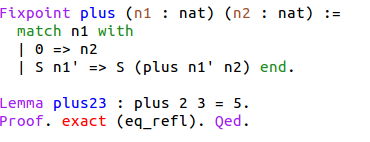
\includegraphics[height = 3cm]{refl.png}
\end{center}


Ce fonctionnement peut être exploité pour construire des preuves qui reposent sur un calcul effectué en Coq. Donnons l'exemple tiré de 


\section{Fonctionnement d'un prouveur automatique}

Utilisation comme boite noire, un des intérêts de l'approche sceptique.\\


SMTLIB, une interface commune aux prouveurs automatiques\\

SAT: \\
cnf : conjonction de clauses \\ 
clause : disjonction de littéraux \\
littéral : atome ou négation d'atome \\
atome : ensemble (fini?) fixé \\

SMT: \\
on peut voir les lemmes de la théorie comme des atomes. Ils sont utilisés par les prouveurs. \\
Fonctionnement d'un smt prouveur :\\
-faire sat sur la formule en considérant les atomes comme indéfinis \\
-en déduire une intanciation qui marche, sinon renvoyer unsat \\
-envoyer cette intanciation aux prouveurs \\
-si tous les prouveurs renvoient vrai alors c'est sat \\
-sinon les prouveurs donnent un lemme additionnel \\
-rajouter ce lemme et recommencer (il y a un nombre fini d'instanciation des atomes)\\ 

Les certificats de veriT:\\
int:(type (clause) dep) \\


Les certificats de zChaff:\\
-maintiennent un état des variables \\
-donnent un ordre d'exécution (L : 2) \\
-définissent des clauses apprises au début du fichier par résolution \\
-définissent des commandes fixant la valeur d'une variable (Var : 5) à vrai (V : 1) ou faux (V : 0) \\
-définissent une clause de conflit (qui explicite les littéraux de conflit)\\

Il y a différentes stratégies pour l'implantation de dpll, on peut choisir de donner une priorité plus importante à la théorie ou aux solveur SAT, à plusieurs niveaux, priorité des règles de Basic dpll. 

La résolution de deux clauses utilise une dérivée de la fonction merge de merge sort.

\newpage 
\section{Présentation de SMTCoq}

\subsection{SMTCoq, une interface sceptique entre Coq et les prouveurs automatiques}

Pour améliorer l'automatisation de Coq et y intégrer l'utilisation de prouveurs automatiques, il y a principalement deux approches.

\begin{multicols}{2}
\begin{center}
Approche autarcique\\
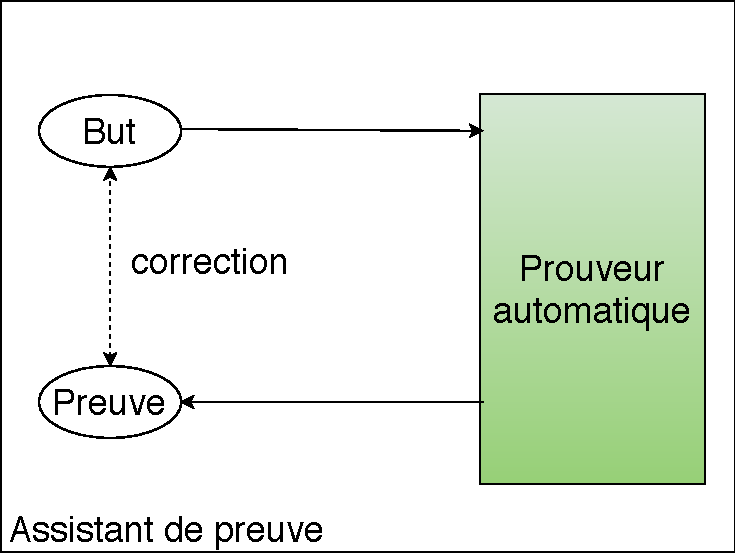
\includegraphics[height=6cm]{1_Autarcique.pdf}\\
Approche sceptique\\
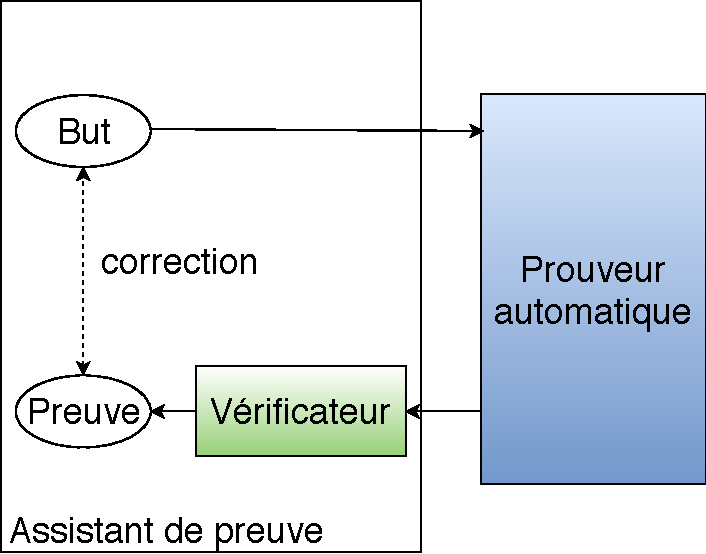
\includegraphics[height=6cm]{2_Sceptique.pdf}\\

\end{center}
\end{multicols}

L'approche autarcique consiste à vérifier le code du prouveur automatique à l'intérieur de l'assistant de preuve. L'avantage de cette méthode est qu'une fois cette vérification faite, on sait que chaque appel du prouveur automatique nous renverra une preuve correcte. \\

Dans l'approche sceptique, le certificat renvoyé par le prouveur automatique est vérifié à chaque appel de celui-ci. Cela permet d'une part de ne pas figer l'implantation du prouveur automatique puisque ce n'est pas son code qui est vérifié mais sa sortie. D'autre part, l'effort de certification est plus restreint : pour un certificat fixé, il faut vérifier que celui-ci correspond bien à une preuve du but.\\

SMTCoq a une approche sceptique de la vérification des prouveurs automatiques.

\subsection{Fonctionnement de SMTCoq}

SCHÉMA CONFIANCE \\

SMTCoq propose une commande de reconstruction de la preuve Coq à partir du certificat fourni par le prouveur automatique. Une fois la reconstruction faite, la vérification que la preuve correspond bien à la proposition de départ est laissée à Coq. \\


SCHÉMA AUTOMATISATION \\

SMTCoq définit également des tactiques Coq, une par prouveur automatique. La tactique "zchaff" par exemple. 

La première étape est la réification. Il s'agit de transformer une formule coq en un AST:
on utilise le terme Ocaml qui représente ce terme Coq.
Cet AST est ensuite envoyé à un prouveur smt, qui nous donne un certificat de preuve.
Il s'agit ensuite de rejouer ce certificat en coq, c'est le vérificateur de SMTCoq.
Il faut pour cela l'interpréter: création de tables qui permettent d'exprimer ce certificat, la formule, les sous-formules apparaissant
dans le certificat, les atomes, les lemmes utilisés. Il y a aussi une étape d'adaptation de ces certificats: il peut manquer des étapes, la forme n'est pas la même que la notre ... \\


Dans les deux cas, les formules acceptées sont les formules logiques propositionnelles en forme prénexe. À cela se rajoute toutes les combinaisons des théories suivantes : arithmétique linéaire sur $\mathbb{Z}$, égalité et fonctions non-interprétées, vecteurs de bits et théories des tableaux. \\

\subsection{Exemples d'utilisation de SMTCoq}

\subsubsection{Exemple de la commande de reconstruction}

SCHÉMA Verit\_Theorem puis Print du théorème créé.

\subsubsection{Exemple de la tactique verit}

SCHÉMA utilisation de verit seulement (pas de print du résultat)


\subsection{Certificats et small checker}
Un certificat est une liste de (certif * position) suivi d'une position finale.\\
Un certif est un type somme de scertif.\\
Un schecker prend un scertif et calcule une nouvelle formule (il faut lui doner l'état aussi).\\
Le checker sera simplement la combinaison par filtrage de ces schecker.
Pour vérifier que le certificat est correct, il faut appliquer dans l'ordre checker sur chacun des certif et modifier la position correspondant à ce certif à chaque étape.\\
Il faut à la toute fin vérifier que la position finale dans l'état est la clause vide.

\subsection{Exemples de certificats et de vérificateurs}
\subsubsection{resolution chains}
C'est simplement une liste de clause.
Le schecker associé fait un fold dessus en appliquant la règle de resolution dessus. Cette règle est
refutationnellement complète.

\subsubsection{nor\_certif}
Il implémente la règle $\neg (A_1 \vee A_2 \vee ... \vee A_n) \Rightarrow ~A_i$

\subsubsection{congruence theory}
Qui implémente les règles de transitivité et de congruence.







\section{Adaptation des certificats}

Afin de ne pas avoir à rajouter des binders dans les proof witness de veriT, nous avons choisi de faire un
preprocessing dans les certificats renvoyés par veriT.
Les règles instance apparaissent sous la forme suivante :
     (forall\_inst (or (not lemma) lemma\_inst) id)
où lemma est un des lemmes rajoutés par l'utilisateur et lemma\_inst est une instance de ce même lemme.

Pour chacune de ces règles instances, on garde une trace du lemme auquel elle se réfère puis on modifie la valeur
de cette règle: ce n'est plus (or (not lemma) lemma\_inst) mais seulement (lemma\_inst). En contrepartie, les règles
de résolution qui utilisent à la fois une de ces règles instances et le lemme associé sont réduites à seulement
l'instance du lemme.

Exemple :
si on a ensuite
(resolution (thm) id1 id2 id3)
et que id2 donne la règle instance écrite ci-dessus et que id3 donne la règle
(input (lemma))
alors on remplace cette règle résolution par une règle de résolution ayant id1 et id2.

On a fait également attention au fait que les règles temporaires de veriT donnent des alias des lemmes de départ
et qu'après une règle forall\_inst il y a une règle qui transforme le OR interne en OR externe.

\renewcommand\refname{Bibliographie
}
\begin{thebibliography}{9}
\bibitem{CIC} 
Christine Paulin-Mohring. Introduction to the Calculus of Inductive Constructions. Bruno Woltzenlogel Paleo; David Delahaye. All about Proofs, Proofs for All, 55, College Publications, 2015, Studies in Logic (Mathematical logic and foundations)

\end{thebibliography}

\end{document}
